\documentclass[]{PLR-ShaofengLiu}
\usepackage{graphicx}
\usepackage{hyperref}


%%%%%%%%%%%%%%%%%%%%%%
%%% Input project details
\def\studentname{Shaofeng Liu}
\def\reportyear{2018}
\def\projecttitle{Literature Review on MSc Project}
\def\supervisorname{Martin R. Albrecht}
\def\degree{MSc in Information Security}

\begin{document}

\maketitle

%%%%%%%%%%%%%%%%%%%%%%
%%% Declaration

\chapter*{Declaration}
I declare that this assignment is all my own work and that I have acknowledged all quotations from published or unpublished work of other people.  I also declare that I have read the statements on plagiarism in Section 1 of the Regulations Governing Examination and Assessment Offences, and in accordance with these regulations I submit this project report as my own work.

\vskip3em

Word Count: 

\vskip3em

Student Name: \studentname

\vskip3em

Date of Submission: 

\vskip3em

Signature:

\newpage


%%%%%%%%%%%%%%%%%%%%%%
%%% Your Abstract here



%%%%%%%%%%%%%%%%%%%%%%
%%% Table of Contents
\tableofcontents\pdfbookmark[0]{Table of Contents}{toc}\newpage
\begin{abstract}
  The first ransomware reviewed to public at 1989 kown as AIDS\cite{AIDS} 
  and then since 2005 the 
  ransomware attack has escalated rapidly with the help of cryptography 
  algorithm. \cite{Symantec:2015}
  GPcode is one of the most famous ransomware family and first version 
  \emph{a} appeared in late 2004.In the year of 2006 version ac appeared and RSA 
  was introduced in the GBcode and the key size after version \emph{ad} has 
  grown very large to defend its encrypted files. \cite{ET,AG}
  For a single year in 2016, 98 new ransomware families was discovered and it is 2 times 
  more than the ransomware family in 2015.\cite{Symantec:2017} 
  Current studies about detecting ransomware have provided effective system
   to capture ransomware but the successful ransomware attack is still one 
   of the most significant threat to individuals and organisations.\cite{ACC}
   And recovery method is highly rely on user's backup.\cite{RHUL:2015}
   The main objective of the project is to provide a detection-recovery 
   hybrid system model and discuss its benefits and limitations. Propose a 
   multiple regression model which evaluate the effectiveness of features 
   and a precise threshold which gives best prediction with low 
   false-positive rate. 
   
\end{abstract}
\newpage




%%%%%%%%%%%%%%%%%%%%%%
%%% Introduction
\chapter{Introduction}
The very first ransomware known as “AIDS Trojan” was implemented by 
Joseph Popp in 1989, after the victims computer been affected AIDS hides 
directories and encrypts the name of all files on drive C: making system 
unusable then pop up a dialog and like many current ransomware it asks 
user to pay to a company called “PC Cybrog Corporation” to renew user’s 
license. With the development of information technology and network 
infrastructure more capable the attacker behind extortion software no 
longer confine to individual user but also commercial companies or other 
organizations, however, the goal of these attackers are mostly the same, 
asking for a payment.\cite{AIDS}

To prevent ransomware from attacker on the delivery stage has always been 
a defensive problem, no matter how hard the security practitioner work the 
adversary always have 0days that never reviewed infiltrate victim’s device 
and taint the system, before the malicious code being activated it remain 
stealth until further instruction therefore a dynamic analysis system is 
important and necessary to capture malicious behavior once the malicious 
code being enabled. 

Ransomware behaves in a different way from traditional malware and such 
differences are the keys to learn its behaviour. Chapter 4 
of this paper will discuss how these behaviours been used to against 
itself.         

Not only personal computer, lots of commercial service has became victim 
of ransomware these days. For example Sony, NHS\cite{CBS:2017} and many 
public service has been attacked by WannaCry and Shamoon Wiper, caused 
delay of public service and even financial loss. The system roll-back and 
recover from back-up image takes long time and effort, to recover from 
ransomware attack normally require victim to wait for the attacker to 
release the sevret key. 23 days average time to resolve a ransomware attack\cite{ACC} is a long 
time for an ordinary user to wait and if a system which is capable of decrypting 
and detecting ransomware at the same time exists, than the damaged system will recover instantly causing less damage.
Current studies about detecting ransomware have provided effective system 
to capture ransomware but the successful ransomware attack is still one of 
the most significant threat to individuals and organisation, during 2017 
the ransomware attack was twice as much as it was in 2016\cite{ACC} and caused 
millions of lost. The recover mechanism provided by Mattias Wecksten, et al. 
highly rely on user’s back up which is not realistic for all users keep 
backup.\cite{IEEE 2nd:2016} By study PayBreak\cite{PayBreak:2017}(A run time recovery system based on study on 
WannaCry) I realised it is possible to combine detection and removal 
mechanism to stop malicious application from damaging the system.

PayBreak is a novel proactive ransomware defensive 
software against WannaCry. In the paper they hook the encryption function 
that custom made for the WannaCry and keep the session keys in a safe 
place then decrypt files after encryption. 

The paper is structured as follows.
In Chapter 3 I will briefly introduce background information and explain the history and different classes of ransomware.
Chapter 4 consists of two parts, the review on previous literature about detecting ransomware and recover from ransomware attack.
In Chapter 5, detailed information about the hybrid system will be presented. Limitations and benefits are discussed in Chapter 6.
Conclude the paper in Chapter7. 

In summary, the main objectives of the project are:
\begin{enumerate}
  \item To get an overview of current literature and technology.
  \item To illustrate the importance and necessity of reducing the ransomware threat.
  \item Provide a regression model using different features
  \item Provide analysis for the experiment on the regression model
  \item Provide a ransomware detection-recovery model
  \item Discussion of the system model
  
\end{enumerate}


\chapter{Preliminary Literature Review}

UNVEIL\cite{UN, UN2}, a novel dynamic analysis system for ransomware detection and behaviour modeling
was proposed in 2016, it is capable of detecting both file locker and screen locker using 
two distinct components. UNVEIL has a filesystem monitoring component which monitoring 
data buffers, I/O requests, process information and screenshots of desktop before, during 
and after execution of the malicious software. The data buffer, I/O request and process 
information is use to compute entropy of a I/O trace, the theory is based on Shannon 
entropy, a file after encryption or compression will have a higher entropy comparing to 
file before encryption. By sorting I/O access request on each file the literature 
believes that a repetitive pattern can be observed on malicious process, in a successful 
malicious attack, an victim file typically been encrypted and overwritten, for some 
variant of ransomware the victim file would be delete or duplicated at some point during 
the malicious process. These operation pattern raise flag of malicious activity on 
filesystem and along with entropy computation UNVEIL has demonstrated it is a high 
precision ransomware detecting system. Not only file locker, UNVEIL is able to detect 
screen locker by taking screenshots of desktop and compute the similarity of the 
screenshots before and after the execution, if the difference has exceeded the threshold 
set by UNVEIL then search ransomware-related text on the image, UNVEIL claims to have 
highest 100\% precision for entire dataset.

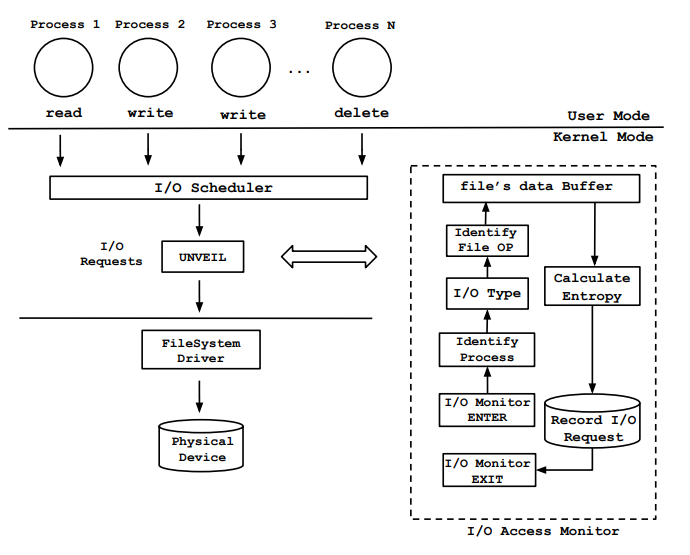
\includegraphics[width=16cm , height=10cm]{UNVEIL.png}
Fig. 1: UNVEIL design overview


The other research team proposed a similar system that dynamically analysis 
and detect ransomware samples by using same indicators and algorithm
(Shannon Entropy), the project is called CryptoDrop\cite{CryptoDrop}. The primary focus of 
this paper is also the behaviour of ransomwares but the difference is in 
this research the develop team uses few more indicators to identify 
malicious process. Recall the UNVEIL computes the entropy of each I/O 
trace and file read/write patterns to identify file locker and screenshots 
for desktop locker, CryptoDrop introduced three primary indicators and two 
secondary indicators and by union these indicators to dynamically identify 
ransomware. The three primary indicators are file type changes, similarity 
measurement and Shannon entropy. These indicators each measure an aspect 
of a file’s transformation, if all three indicators has been met then a 
file is likely to have a ransomware-related transformation. The analysis 
on file operation is more detailed compare to UNVEIL because UNVEIL 
observe read/write operation patterns but these pattern is likely to be 
evaded or a innocent process doing harmless operations. For example the 
attacker could pad user file with low entropy bytes to lower the post 
encryption entropy and a normal user process is merging file content to 
original one. CryptoDrop records type change of files and bulk 
modifications to raise red flag, but a update of software will have the 
same “suspicious” activity therefore second indicator is used to prevent 
this false-positive from happening, by using similarity-preserving hash 
function to compare a file before and after modification to observe any 
suspicious activities, one characteristic of a good encryption algorithm 
is that the cipher text should not review any information from plaint 
text, although updating file could broadly change the content, the 
difference will not be as huge as a encryption process and dissimilarity 
of new file to original file give the system enough reason to suspect the
 process. Research shows that English text has fairly low entropy because 
 it is easy to predict, after encryption or compression the entropy will 
 be higher because the text contains more higher information per character, 
 thus, if the file has been modified by a process and has higher entropy 
 this entropy indicator will later help to classify the malware sample. 
 File deletion gives little less information on file transformation 
 because not all ransomware delete or unlink user files and benign may 
 create temporary file and delete it but mass deletion of file is 
 indicates some degree of malicious activities. File type funneling occurs 
 when application reads unusual large amount of files as it writes, it is 
 normal for example a Microsoft Word allow user to attach pictures, audios 
 and other’s document but only output a single document but for a success 
 ransomware attack, the malicious application will output as much file as 
 it reads for a board range of data type. The CryptoDrop state that none 
 of its benign sample has triggered all three primary indicators while 
 vast majority of ransomware does. CryptoDrop claim to have 100\% 
 detection rate same as UNVEIL. 

Unlike previous researches using controlled environment to analysis 
malicious application, Daniel Nieuwenhuizen\cite{MWR} from MWR Lab proposed a 
machine learning approach to detect and classify ransomware, in the 
research the author has stated that ransomware detection requires a 
decision making algorithm which is the result of supervised-machine 
training and such training process need three crucial components: 
application samples dataset (both malicious and benign), behavioural 
indicator which can be quantified for example file entropy trace and 
a classification which defines training and prediction algorithm, 
although the research does not show large number of experiment data, 
it shows the ability of predict a 0day ransomware.

An earlier research\cite{RHUL:2015, Lorenzo:RHUL, DDH:2015} proposed a ransomware detection and dynamic analysis 
system which implemented machine learning component to classify ransomware 
and ordinary applications, their machine learning component	consists a 
feature selection phase which select the most discriminating features to 
pass into the Regularized Logistic Regression classifier. The live 
detection component gathers samples from network from both legitimate 
website and malicious source such as phishing emails, EldeRan then extract 
features from these sample and by the help of the classifier the program 
will output whether the application is malicious.
The classification features EldeRan uses is mainly focused on system operations and static information while UNVEIL and CryptoDrop primary focus is the information that carried by the file.
  \begin{enumerate}
    \item Windows API calls (i.e., the traces of invocations of native
      functions and Windows API calls).
    \item Registry Key Operations (in particular, the read, open, write, and delete
operations).
    \item File System Operations (in particular, the read, open, write, and delete operations).
    \item the set of file operations performed per File Extension. 
    \item Directory Operations (the set of operations performed on directories,
in particular the enumeration and creation).
    \item Dropped Files (i.e., the set of files that are dropped by an application
during installation).
    \item Strings (the strings embedded in the binary). 
  \end{enumerate}

 
 

Mattias Wecksten, et al.\cite{IEEE 2nd:2016} has proposed a method to 
recover from crypto ransomware infection by renaming a system process 
vssadmin.exe (which is necessary for Windows system recovery) and recover 
after a successful ransomware attack, this method requires victim maintain 
a proper backup scheme therefore to minimize the damage but if the data is 
updated in a short time frame with high frequency then this method will 
only recover the system but not preventing data lost fully the result of 
recovery is highly rely on user’s behaviour.

Take a recent example of ransomware attack: WannaCry\cite{UN2,Secureworks} 
which caused the hospital in the UK paralysed for a short period and 
over 100,000 personal device been affected. PayBreak\cite{PayBreak:2017} 
was designed to recover from the damage caused by this crypto-based 
ransomware,  WannaCry uses self-compiled AES-128-CBC cryptography system 
to generate keys to encrypt infected files. The idea of this program is 
to monitor the keyGen() and the victim filesystem, record the key 
generated and corresponding file and keep this record in an “vault” 
and this key-file pair will be used to recover file after the attack. 
It does not rely on user’s backup and the author also stated that it 
is unrealistic for all user to use backups. And given the significant growth 
of ransomware attacks to personal computer\cite{Symantec:2017, ACC}, I believe
that to reduce the lost of property ransomware needs to be detected, terminated and recovered
more efficiently.
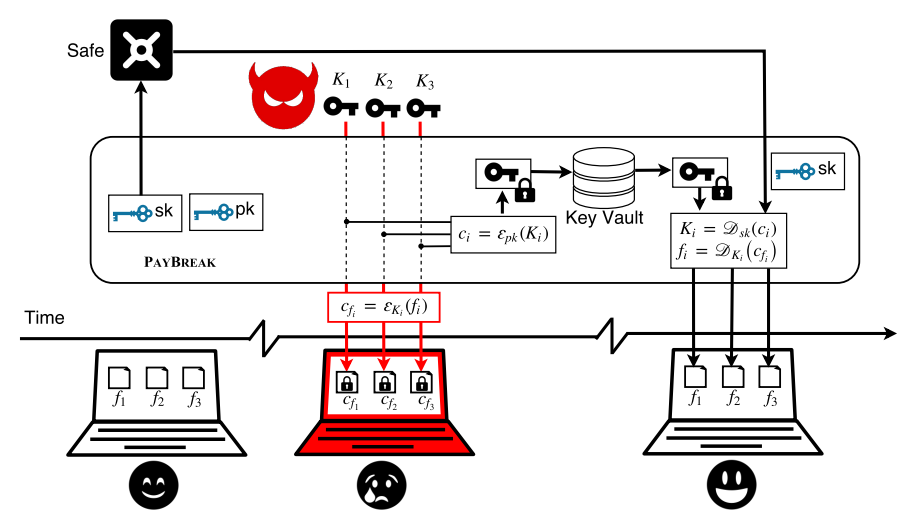
\includegraphics[width=16cm , height=10cm]{paybreak.png}
                        Fig.2: PayBreak's process flow

By reviewing literature, I realise that many effective systems have been 
developed to detect and analysis ransomware while recovering system has 
very little improvement. PayBreak has demonstrated the ability to defeat 
most ransomware families but as process flow diagram shown, the decrypting 
mechanism will not work until ransomware finish encryption and if malware 
is specifically aiming to evade or overwrite PayBreak’s executable file 
then the decryption will not work after the encryption. Thus I believe 
that detection system running simultaneously is necessary, stopping 
malicious code before it finishes attack system potentially reduce 
the recover time and gives another layer of protection to defend the system for 
a successful attack which managed to infiltrate the system.

The indicators CryptoDrop\cite{CryptoDrop} has introduced to detect ransomware 
demonstrated strong ability to detect ransomware activity and merging these indicators with
other features used by other similar\cite{UN, UN2} or machine-learning based system\cite{RHUL:2015,Lorenzo:RHUL}
in one model could potentially benefits the outcome of ransomware detection, therefore an experiment
will be conduct in the proposed paper to identify any improvement or deterioration.







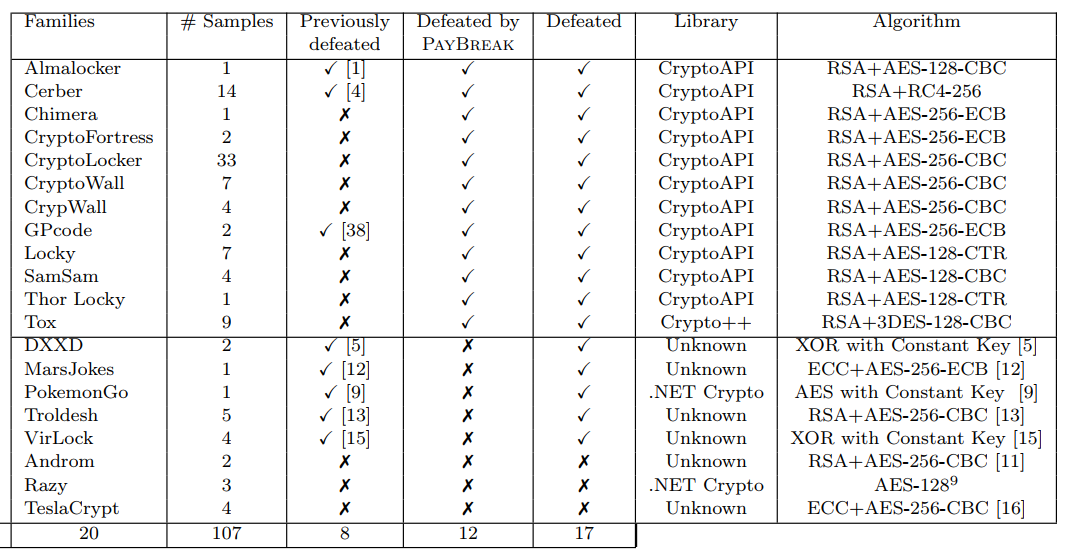
\includegraphics[width=16cm , height=10cm]{paybreak_r.png}
Fig.3: Ransomware samples

\section{Methodology}
Many approaches have been proposed recent year that aiming to analysis and detect malicious software. The primary research method for the system model is literature review and extract component which can be implemented in the system model. The thesis will first review various types of detection study such as dynamic-behaviour analysis and machine learning based behaviour analysis(Dynamic and static). I obtain available literature through on-line resources(search engine, IEEE) and public research projects. Tools which help to finish the experiment part of the project, for example, file generators, file change monitor from GitHub.

Based on the understanding of previous literature, a multiple regression model will be developed to help modeling the hybrid system, in this stage of study, ransomware dataset is needed for the regression model but variables for the model are missing from the datasets(i.e file entropy value before and after attack), therefore experiment on ransomware sample will be necessary in order to obtain the mean entropy of each ransomware family.

The dataset obtained has 582 samples of ransomware and 942 benign applications, 10 ransomware families, 7 sets of features and total of 30970 features. The 7 sets of features are:

  \begin{enumerate}

    \item API API invocations
    \item DROP Extensions of the dropped files
    \item REG Registry key operations
    \item FILES File operations
    \item FILES\_EXT Extension of the files involved in file operations.
    \item DIR File directory operations
    \item STR Embedded strings
          
  \end{enumerate}
  This project is mainly focus on file system operations therefore the STR set and 
  REG set will be ignored, and other features such as API:closesocket and API:Http* 
  will be dropped from the dataset. 
Shannon’s entropy will be added to the dataset as a new feature, entropy value 
indicates the information carried by the file, compression and encryption operation 
on raw file will make the resulting file has higher entropy than before. The entropy 
e of a file can be computed as:

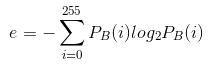
\includegraphics{entropy.png}

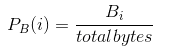
\includegraphics{entropy1.png}

Bi it the number of byte value i in the byte array, this will produces e from range 0 to 8, because the maximum information a byte can carry is 8-bits.
The dataset will be processed and visualized in R-studio because it has powerful regression library and provide easy manipulation to dataset. The summary() function returns useful information such as F-statistic and T-value for optimizing the regression model. The regression model denotes as:
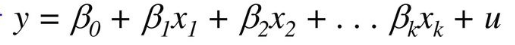
\includegraphics{MRR.png}

Where Xi is the selected features(i.e entropy, number of file deleted).
The experiment will be carried out in Windows system on top of an open source malware analysis Cuckoo Sandbox, generating random files with extensions which the most common to user in a designated directory then calculate the average entropy before and after attack as the new feature to the ransomware sample. Due to the scope and time frame of the project monitoring entire file system is not feasible. The program will be written in JAVA.
\newpage
\chapter{Ransomware}
Ransomware is a piece of malicious software that once infiltrated and 
installed in personal computer, it takes full control of the device then 
threat user with damaging files, denial of access to data or operating 
system. Ransom payment is demanded by the attacker in exchange of unlock 
the victim device(s), however the promises are not always fulfilled. A 
traditional malicious software typically would remain stealth after  its 
been delivered to victims system and even when it is triggered, 
the code itself is designated to draw less attention from system and 
victim in order to steal information such as bank details, keystrokes 
of password or using victims device as Bitcoin mining machine. 
In contrast, the goal of ransomware need it to behave in an opposite way, 
the malicious code will  notify  user  directly  that  user  being  hacked.
  \section{How Ransomware get installed}
  
  \section{Types of Ransomware}
\chapter{Defending Ransomware}
  \section{Detecting Ransomware}
    \subsection{Dynamic behaviour analysis}
    \subsection{Machine learning approach}
  \section{Recover from Ransomware}
\chapter{A hybrid system model}
  \section{System design}
    \subsection{Machine learning based detection module}
        \subsubsection{Multiple Regression Model}
        \subsubsection{Analysis of the features}
        \subsubsection{Experiment and Optimisation}
        \subsubsection{Result} 
      \subsection{Recover component}
  \section{System requirements}
  \section{Execution flow}
\chapter{Discussion}
  \section{Benefit}
  \section{Limitations}
\chapter{Conclusion}


%%%% ADD YOUR BIBLIOGRAPHY HERE
\newpage

\begin{thebibliography}{99}
\addcontentsline{toc}{chapter}{References}
\bibitem{UN} Amin Kharaz, Sajjad Arshad, Collin Mulliner, William Roberson and Engin Kirda. \emph{UNVEIL: A Large-Scale, Automated Approach
to Detecting Ransomware}. USENIX Security Symposium. 2016: [757-772].
\bibitem{CBS:2017}CBS Interactive Inc. \emph{Global cyberattack strikes dozens of countries, cripples U.K. hospitals}. https://www.cbsnews.com/news/hospitals-across-britain-hit-by-ransomware-cyberattack/
\bibitem{PayBreak:2017}Eugene Kolodenker, William Koch, Gianluca Stringhini, and Manuel Egele.\emph{PayBreak : Defense Against Cryptographic Ransomware}.Proceedings of the 2017 ACM on Asia Conference on Computer and Communications Security [599--611]
\bibitem{MWR}Daniel Nieuwenhuizen.\emph{A behavioural-based approach to ransomware detection}. https://labs.mwrinfosecurity.com/publications/a-behavioural-based-approach-to-ransomware-detection/
\bibitem{CryptoDrop}Nolen Scaife, Henry Carter, Patrick Traynor, Kevin R.B Butler. \emph{CryptoLock (and Drop It):
Stopping Ransomware Attacks on User Data}. 2016 IEEE 36th International Conference on Distributed Computing Systems [303-312] 
\bibitem{IEEE 2nd:2016}Mattias Weckst\'en, Jan Frick, Andreas Sj\"ostr\"om, Eric J\"arpe.\emph{A Novel Method for Recovery from Crypto Ransomware Infections }Computer and Communications (ICCC), 2016 2nd IEEE International Conference on. IEEE, 2016: [1354-1358].
\bibitem{Lorenzo:RHUL}Roberto Jordaney+, Kumar Sharad§, Santanu Kumar Dash‡, Zhi Wang†, Davide Papini•, Ilia Nouretdinov+, and Lorenzo Cavallaro+.\emph{Transcend: Detecting Concept Drift in Malware Classification Models}.Proceedings of the 26th USENIX Security Symposium (USENIX Security 2017). 2017.[625--642]
\bibitem{Secureworks}COUNTER THREAT UNIT RESEARCH TEAM. \emph{WCry Ransomware Analysis}. www.Secureworks.com
\bibitem{CSV:2017}Menlo Park. \emph{Ransomware Damage Report}. CybersecurityVentures.com
\bibitem{Kh} Amin Kharraz and William K. Robertson and Davide Balzarotti and Leyla Bilge and Engin Kirda. \emph{Cutting the Gordian Knot: A Look Under the Hood of Ransomware Attacks}. Detection of Intrusions and Malware, and Vulnerability Assessment,2015, p3-24
\bibitem{Yang:2015} Tianda Yang and Yu Yang and Kai Qian and Dan Chia-Tien Lo and Ying Qian and Lixin Tao. \emph{Automated Detection and Analysis for Android Ransomware}. 2015 IEEE 17th International Conference on High Performance Computing and Communications, 2015 IEEE 7th International Symposium on Cyberspace Safety and Security, and 2015 IEEE 12th International Conference on Embedded Software and Systems[1338-1343]
\bibitem{RHUL:2015}Daniele Sgandurra, Luis Muñoz-González, Rabih Mohsen, Emil C. Lupu. \emph{Automated Dynamic Analysis of Ransomware:
Benefits, Limitations and use for Detection}. arXiv preprint arXiv:1609.03020
\bibitem{DDH:2015}Diane Duros Hosfelt. \emph{Automated detection and classification
of cryptographic algorithms in binary
programs through machine learning}.arXiv preprint arXiv:1503.01186, 2015.
\bibitem{Symantec:2017} Symantec. \emph{2017 Internet Security Threat Report}. https://www.symantec.com/security-center/threat-report.
\bibitem{UN2}Qian Chen, Robert A. Bridges. \emph{Automated Behavioral Analysis of Malware
A Case Study of WannaCry Ransomware}. 2017 16th IEEE International Conference on Machine Learning and Applications.
\bibitem{AIDS}A. Young and Moti Yung, \emph{Cryptovirology: extortion-based security threats and countermeasures}. Proceedings 1996 IEEE Symposium on Security and Privacy, Oakland, CA, 1996, pp. 129-140.
\bibitem{Symantec:2015}Kevin Savage, Peter Coogan, Hon Lau \emph{The evolution of Ransomware}. https://www.symantec.com/content/dam/symantec/docs/security-center/white-papers/the-evolution-of-ransomware-15-en.pdf
\bibitem{AG}Alexandre Gazet.\emph{Comparative analysis of various ransomware virii}. Journal in computer virology, 2010, 6(1): [77-90].
\bibitem{ET}Eran Tromer. \emph{Cryptanalysis of the Gpcode.ak ransomware virus}. https://rump2008.cr.yp.to/6b53f0dad2c752ac2fd7cb80e8714a90.pdf
\bibitem{ACC}ACCENTURE.\emph{COST OF CYBER CRIME 2017}. https://www.accenture.com



\label{endpage}
\end{thebibliography}




\end{document}

\end{article}
